\section{Stosowane rozwiązania}
W trakcie realizacji projektu Poznańskie Nowe Zoo dysponowało kilkoma
inkubatorami, pozwalającymi na inkubację łącznie około 200 jaj o~rozmiarach od
pustułczych do strusich. Urządzenia te zostały zakupione w~przeciągu ostatnich
20 lat i~stosują wiele nieaktualnych rozwiązań, posiadają liczne wady
i~ograniczenia. Stosują one sterowanie liniowe. Zadane wartości \emph{sterowanych
parametrów} (temperatury, wilgotności, częstości obracania jaj) ustawia się
w~nich przy pomocy pary analogowych pokręteł, co jest nieprecyzyjne. Co więcej,
pokrętła są podatne na przypadkowe zmiany pozycji i~trudno jest z~nich odczytać
faktycznie nastawione wartości. Absurdalną sytuację zaobserwowano, gdy
pracownicy Zoo kreślili po obudowie inkubatora, aby zapamiętać jakie powinny być
położenia pokręteł. Aktualną temperaturę w~stosowanych
inkubatorach można zweryfikować jedynie poprzez odczytanie wskazania rtęciowego
termometru umieszczonego wewnątrz inkubatora. Analogowe metody pomiarów
i~sterowania są niedoskonałe i~podatne na wzrost błędu wraz z~czasem życia
urządzenia. Niektóre inkubatory wymagały też regularnej interwencji personelu
w~celu obrócenia jaj.

Nowoczesne inkubatory \cite{Brinsea} \cite{Metzer} rozwiązują część z~powyższych problemów. Posiadają takie
cechy jak elektroniczne sterowanie temperaturą, wilgotnością i~wentylacją oraz
niezależne cyfrowe termometry gwarantujące obiektywny odczyt. Niektóre
rozwiązania wyposażone są w~alarm informujący o~zbyt wysokiej lub zbyt niskiej
temperaturze czy też awarii zasilania, a~także posiadają w~pełni automatyczny
mechanizm obracania jaj, poprzez rotację komory inkubacyjnej.

Mimo postępu technologii zarówno w~starszych inkubatorach jak i~w urządzeniach najnowszych programowanie działania inkubatora ogranicza się do zadania stałej wartości
sterowanym parametrom. Tymczasem możliwość zaprogramowania zmiennej w~czasie
funkcji temperatury lub wilgotności jest bardzo pożądana przez ornitologów.
Podczas inkubacji niektórych gatunków co kilka dni trzeba zmieniać ręcznie
ustawienia temperatury i~wilgotności. Ponadto w~celu symulowania warunków
naturalnych co kilka godzin wietrzy się inkubatory na kilkanaście minut.
%[[ symulując sytuację, gdy wysiadujący ptak schodzi z~jaj. ]]
W~istniejących rozwiązaniach brakuje też możliwości rejestracji przebiegu
inkubacji. Aby upewnić się, że urządzenie w~danej chwili działa prawidłowo,
ornitolog musi odczytać wartości sterowanych parametrów bezpośrednio
z~inkubatora. W~przypadku nieudanej inkubacji, czyli niskiej klujności zdrowych
zalążków, niemożliwa jest ocena przyczyn niepowodzenia. W~szczególności, nie
można powiedzieć, czy zawiniły błędy teoretyczne, czyli niewłaściwie dobrane
wartości sterowanych parametrów, czy błędy techniczne, jak np. nocna awaria
zasilania. Te ograniczenia znacznie utrudniają prowadzenie badań naukowych na
temat inkubacji.

Projekt Thinkubator ma za zadanie wprowadzić nową jakość do procesu inkubacji.
Ma on umożliwiać programowanie dowolnej zmienności wszystkich sterowanych
parametrów inkubacji w~czasie. W~prosty sposób da możliwość nastawienia chłodzenia,
dobowych wahań temperatury oraz automatycznego rolowania. Po zaprogramowaniu
inkubatora system będzie nieustannie monitorować proces inkubacji, co będzie umożliwiać
sprawdzenie przebiegu procesu zarówno w~trakcie jego trwania jak i~po jego
zakończeniu. Dzięki temu będzie to jedyny system, który w~takim stopniu wspiera
badania naukowe nad inkubacją zagrożonych gatunków. Dodatkowo system umożliwi
zdalny monitoring inkubatora przez Internet oraz stworzenie mechanizmu szybkich
powiadomień w~przypadku awarii zasilania lub innych niepożądanych zdarzeń.
Będzie pozwalać na współdzielenie doświadczeń z~innymi jego użytkownikami, przez co
umożliwi nawiązywanie współpracy ornitologom z~różnych ogrodów zoologicznych. Ze
współdzielenia informacji będą mogli korzystać również ornitolodzy-amatorzy,
ponieważ narzędzie do programowania inkubacji zaproponuje użytkownikowi
optymalne wartości sterowanych parametrów, nawet przy jednoczesnej inkubacji jaj
różnych gatunków.

\section{Cel projektu}
Celem projektu jest stworzenie systemu do inkubacji jaj ptasich w~kontrolowanym
środowisku. System ten składa z~urządzenia pozwalającego na inkubację jaj
w~warunkach identycznych z~naturalnymi oraz podsystemu informatycznego,
odpowiedzialnego za kontrolę i~analizę procesu inkubacji. Ogólny schemat
połączeń między urządzeniami został przedstawiony na rysunku
\ref{rys:SystemDiagram}.

\subsection{Wizja systemu}
Urządzenia wchodzące w~skład systemu Thinkubator podzielone są na trzy poziomy:

\begin{figure}[t] 
\centering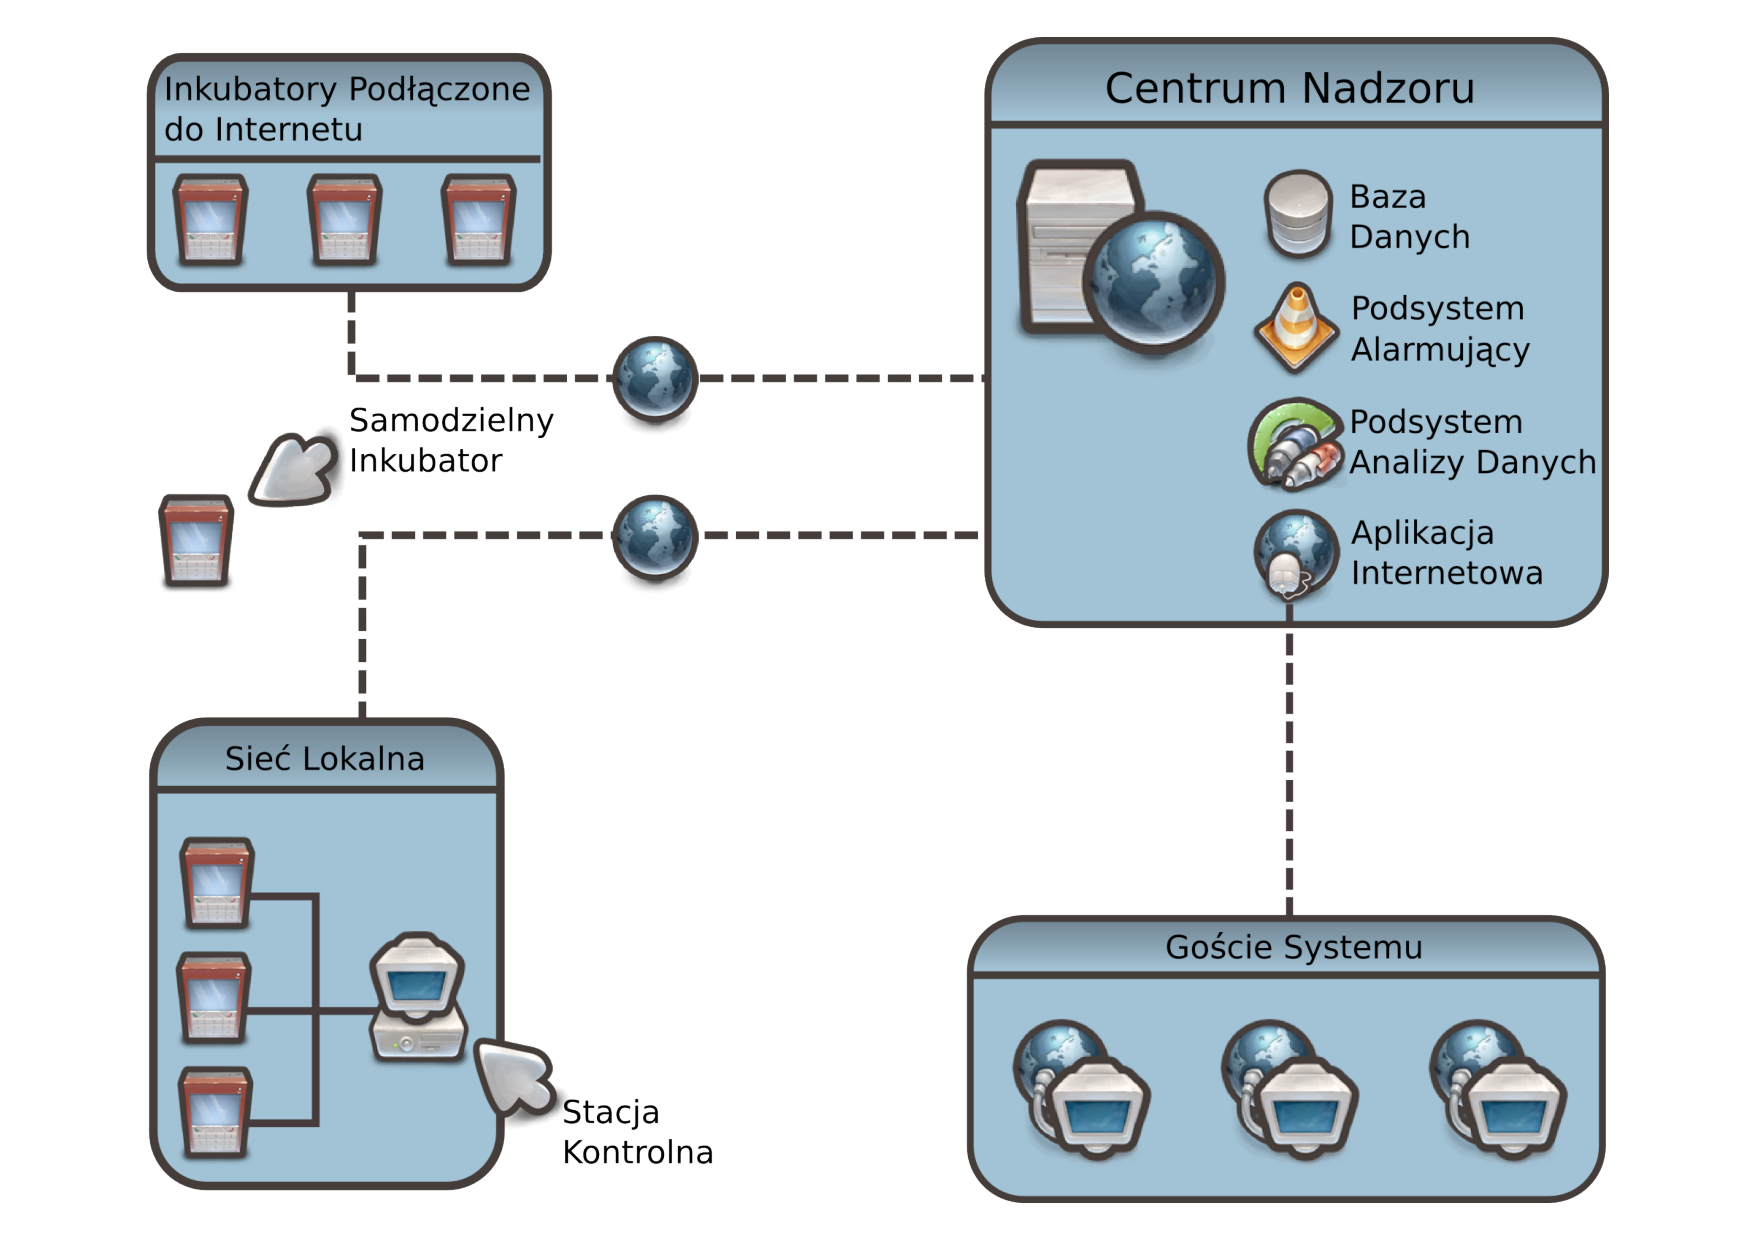
\includegraphics[width=\textwidth]{figures/System_Diagram}
\caption{Diagram systemu}\label{rys:SystemDiagram}
\end{figure}

\paragraph{Poziom 1. -- Inkubator.}
Najważniejszy element systemu. Pozwala na inkubację jaj oraz monitorowanie
tego procesu. Jako samodzielnie urządzenie posiada pełną funkcjonalność typowego
inkubatora. Dodatkowo wyposażony jest w~klawiaturę oraz wyświetlacz LCD,
pozwalające w~intuicyjny sposób programować inkubator oraz wyświetlać aktualne
wartości sterowanych parametrów.

\paragraph{Poziom 2. -- Stacja Kontrolna.}
Komputer połączony z~inkubatorami siecią lokalną Ethernet. Pozwala ornitologom
na zaprogramowanie inkubatora. Pomaga w~doborze optymalnych wartości sterowanych
parametrów w~przypadku jednoczesnej inkubacji jaj różnych gatunków. Na bieżąco
monitoruje i~wizualizuje parametry trwających oraz zakończonych inkubacji.

\paragraph{Poziom 3. -- Centrum Nadzoru.}
Zdalny serwer pracujący non-stop. Składa się z~następujących podsystemów:
\begin{itemize}
	\item bazy danych, która gromadzi informacje o~przebiegu oraz efektywności
		inkubacji ze wszystkich zarejestrowanych w~systemie inkubatorów oraz
		przechowuje wyniki analizy danych,
	\item podsystem alarmowania -- w~równych odstępach czasu rejestruje stan
		wszystkich inkubatorów, a~w~przypadku wykrycia błędnego stanu podejmuje
		odpowiednie działania alarmujące,
	\item podsystem analizy danych -- narzędzia do analizy wpływu warunków
		inkubacji (np. średniej temperatury, najdłuższego czasu bez zasilania) na
		klujność; funkcjonalność ta została zaprojektowana z~myślą o~rozszerzeniu systemu w~przyszłości,
	\item podsystem wizualizacji -- aplikacja internetowa służąca do nadzoru
		systemu i~wizualizacji przechowywanych danych,
	\item podsystem administracyjny -- panel służący do zarządzania inkubatorami.
\end{itemize}

Poszczególne elementy systemu zostały tak zaprojektowane by ściśle
współpracowały z~urządzeniami na niższym poziomie, natomiast były niezależne od
urządzeń na wyższym poziomie. Pozwala to na poprawne działanie systemu
w~przypadku gdy jest on ograniczony do dwóch poziomów (Inkubator i~Stacja
Kontrolna, Inkubator i~Centrum Nadzoru) lub tylko jednego poziomu (Inkubator).
Dodatkowo uniezależnienie poziomów pozwala na zwiększenie niezawodności
systemu oraz zapewnia odporność na utratę danych w~wyniku awarii urządzenia na
niższym poziomie.

\subsection{Zasady działania systemu}
Poniższy scenariusz opisuje ogólny sposób wykorzystania systemu:
\begin{itemize}
	\item Proces inkubacji rozpoczynany jest poprzez umieszczenie w~inkubatorze
		jaj i~zaprogramowanie inkubatora przy pomocy wbudowanej klawiatury lub
		Stacji Kontrolnej. Inkubacja trwa od dwóch tygodni do dwóch miesięcy.
		W~dowolnej chwili można zmienić ustawiony program inkubacji.
	\item Przy programowaniu inkubatora Stacja Kontrolna wyświetla dostępne wzorce
		inkubacji pomagając w~optymalnym doborze sterowanych parametrów.
	\item Stacja Kontrolna regularnie pobiera uaktualnienia wzorców inkubacji
		w~Centrum Nadzoru.
	\item Wartości wszystkich sterowanych parametrów inkubacji są przechowywane
		w~pamięci inkubatora i~mogą być odczytane przez Stację Kontrolną.
	\item Wiadomości kontrolne z~wartościami sterowanych parametrów są wysyłane do
		Stacji Kontrolnej i~Centrum Nadzoru w~równych odstępach czasu.
	\item Ornitolog może sprawdzić stan procesu inkubacji na trzy sposoby (trzy
		poziomy kontroli):
		\begin{itemize}
			\item odczytując wskazania na cyfrowym wyświetlaczu inkubatora,
			\item przy pomocy Stacji Kontrolnej, która wyświetla bieżące wartości
				sterowanych parametrów dla wszystkich działających inkubatorów w~sieci
				lokalnej,
			\item po zalogowaniu do Centrum Nadzoru, do którego ma dostęp z~każdego
				miejsca na świecie.
		\end{itemize}
	\item W~przypadku błędnego stanu inkubacji uruchamiane są trzy sposoby
		alarmowania odpowiadające poziomom kontroli:
		\begin{itemize}
			\item Inkubator -- alarm dźwiękowy,
			\item Stacja Kontrolna -- wyświetlenie powiadomienia,
			\item Centrum Nadzoru -- powiadomienie e-mailowe, możliwość dodania
				funkcjonalności powiadomień sms-owych.
		\end{itemize}
	\item Centrum Nadzoru gromadzi informacje o~przebiegach inkubacji w~celu
		współdzielenia doświadczeń i~analizy danych.
	\item Za przyzwoleniem ogrodu zoologicznego informacja o~stanie inkubatora
		może być udostępniona anonimowym użytkownikom aplikacji internetowej
		w~Centrum Nadzoru. Pozwoli to na zwiększenie zainteresowania użytkowników
		Internetu pracami prowadzonymi w~zoo i~zachęci ich do odwiedzenia ogrodu.
\end{itemize}

\subsection{Opis funkcjonalności systemu}
Poszczególne części systemu thinkubator pełnią następujące funkcje:

\noindent\textbf{Inkubator}:
\begin{itemize}
	\item zapewnienie optymalnych warunków inkubacji poprzez jak najwierniejsze
		odtworzenie rzeczywistych warunków inkubacji,
	\item sterowanie w~zakresie temperatury, wilgotności i~obracania jaj,
	\item wyświetlanie na wyświetlaczu LCD parametrów inkubacji,
	\item możliwość zaprogramowania inkubacji przy pomocy wbudowanej klawiatury,
	\item możliwość zaprogramowania inkubacji przy pomocy Stacji Kontrolnej,
	\item zbieranie danych pomiarowych,
	\item rozsyłanie danych pomiarowych do Stacji Kontrolnej i~Centrum Nadzoru.
\end{itemize}
\textbf{Stacja Kontrolna}:
\begin{itemize}
	\item jednoczesne monitorowanie wszystkich inkubatorów w~sieci,
	\item wizualizacja przebiegu sterowanych parametrów inkubacji w~funkcji czasu
		przez cały okres inkubacji,
	\item programowanie inkubatora,
	\item pomoc w~doborze nastaw poprzez wizualizację wzorców inkubacji jaj
		jednego lub wielu różnych gatunków,
	\item pobieranie uaktualnień wzorców z~Centrum Nadzoru,
	\item przechowywanie danych o~przebiegu inkubacji w~celu wizualizacji lub
		wysłania ich do Centrum Nadzoru.
\end{itemize}
\textbf{Centrum Nadzoru}:
\begin{itemize}
	\item gromadzenie danych z~przebiegu inkubacji (zaprogramowane i~rzeczywiste
		wartości sterowanych parametrów),
	\item monitorowanie bieżącego stanu inkubatorów,
	\item wizualizacja przebiegu wartości sterowanych parametrów dla każdej
		inkubacji,
	\item analiza danych w~celu tworzenia wzorców,
	\item alarmowanie o~błędach,
	\item uwierzytelnianie i~autoryzacja użytkowników -- kontrola dostępu do
		poszczególnych funkcji systemu,
	\item zarządzanie kontami użytkowników.
\end{itemize}

\subsection{Wymagania wydajnościowe}
Mimo szerokiej funkcjonalności systemu Thinkubator, podstawowym wymogiem jakie
musi on spełniać jest zapewnianie odpowiednich warunków inkubacji w~komorze
inkubacyjnej. Inkubator musi zagwarantować sterowanie temperaturą z~dokładnością
przynajmniej~0,3\st{} (optymalnie~0,1\st) oraz wilgotnością z~dokładnością do~5\%
względnej wilgotności (optymalnie~1\%). Komora inkubacyjna powinna pomieścić
około~50 jaj i~być szczelna aby nie dopuszczać do wahań temperatury i~wilgotności.
Wnętrze komory musi być wietrzone by zapewnić świeży dopływ tlenu
oraz nie dopuścić do nadmiernego wzrostu wilgotności. Aby idealnie odwzorowywać
warunki naturalne inkubator musi być wyposażony w~mechanizm obracania jaj.
